\documentclass[a4paper, 14pt]{extarticle}
\usepackage[utf8]{inputenc}
\usepackage[paper=a4paper, top=1cm, right=1cm, bottom=1.5cm, left=2cm]{geometry}
\usepackage{setspace}
\onehalfspacing

\usepackage{graphicx}
\graphicspath{{plots/}, {images/}}

\parindent=1.25cm

\usepackage{titlesec}

\titleformat{\section}
    {\normalsize\bfseries}
    {\thesection}
    {1em}{}

\titleformat{\subsection}
    {\normalsize\bfseries}
    {\thesubsection}
    {1em}{}

% Настройка вертикальных и горизонтальных отступов
\titlespacing*{\chapter}{0pt}{-30pt}{8pt}
\titlespacing*{\section}{\parindent}{*4}{*4}
\titlespacing*{\subsection}{\parindent}{*4}{*4}

\usepackage[square, numbers, sort&compress]{natbib}
\makeatletter
\bibliographystyle{unsrt}
\renewcommand{\@biblabel}[1]{#1.} 
\makeatother


\newcommand{\maketitlepage}[6]{
    \begin{titlepage}
        \singlespacing
        \newpage
        \begin{center}
            Министерство образования и науки Российской Федерации \\
            Федеральное государственное бюджетное образовательное \\
            учреждение высшего профессионального образования \\
            <<Волгоградский государственный технический университет>> \\
            #1 \\
            Кафедра #2
        \end{center}


        \vspace{14em}

        \begin{center}
            \large Семестровая работа #6 по дисциплине
            \\ <<#3>>
        \end{center}

        \vspace{5em}

        \begin{flushright}
            \begin{minipage}{.35\textwidth}
                Выполнила:\\#4
                \vspace{1em}\\
                Проверил:\\#5
                \\
                \\ Оценка \underline{\ \ \ \ \ \ \ \ \ \ \ \ \ \ \ \ }
            \end{minipage}
        \end{flushright}

        \vspace{\fill}

        \begin{center}
            Волгоград, \the\year
        \end{center}

    \end{titlepage}
    \setcounter{page}{2}
}

\newcommand{\maketitlepagewithvariant}[7]{
    \begin{titlepage}
        \singlespacing
        \newpage

        \begin{center}
            Министерство образования и науки Российской Федерации \\
            Федеральное государственное бюджетное образовательное \\
            учреждение высшего профессионального образования \\
            <<Волгоградский государственный технический университет>> \\
            #1 \\
            Кафедра #2
        \end{center}


        \vspace{8em}

        \begin{center}
            \large Семестровая работа #6 по дисциплине
            \\ <<#3>>
        \end{center}

        \vspace{1em}
        \begin{center}
            Вариант №#7
        \end{center}
        \vspace{4em}

        \begin{flushright}
            \begin{minipage}{.35\textwidth}
                Выполнила:\\#4
                \vspace{1em}\\
                Проверил:\\#5
                \\
                \\ Оценка \underline{\ \ \ \ \ \ \ \ \ \ \ \ \ \ \ \ }
            \end{minipage}
        \end{flushright}

        \vspace{\fill}

        \begin{center}
            Волгоград, \the\year
        \end{center}

    \end{titlepage}
    \setcounter{page}{2}
}

\input{../../.preambles/10-russian}
\input{../../.preambles/20-math}
\input{../../.preambles/22-vectors}
\input{../../.preambles/30-physics}
\usepackage{mathrsfs}

\renewcommand{\labelenumi}{\asbuk{enumi})}
\renewcommand{\mid}[1]{\left\langle #1 \right\rangle}
\newcommand{\ds}{\displaystyle}
\newcommand{\inv}{\mathrm{inv}}
\renewcommand{\v}{\mathrm{v}}
\newcommand{\E}{\mathscr{E}}

\begin{document}
\maketitlepage{Факультет электроники и вычислительной техники}
{физики}{Электродинамика}{студентка группы Ф-369\\Слоква~В.~И.}
{доцент Грецов~М.~В.}{№3}

Задача 1.14: \emph{Определить поле плоского конденсатора, обкладки которого
равномерно заряжены с поверхностной плотностью зарядов \( +\sigma \) и
\( -\sigma \). Пространство между ними заполнено неоднородным диэлектриком,
проницаемость которого \( \eps = \eps(x) \). Краевым эффектом пренебречь. Ось
\( x \) направлена перпендикулярно к обкладкам от положительно заряженной
обкладки к отрицательной.}

\vspace*{2em}
\emph{Решение:}

\begin{minipage}{.4\textwidth}
    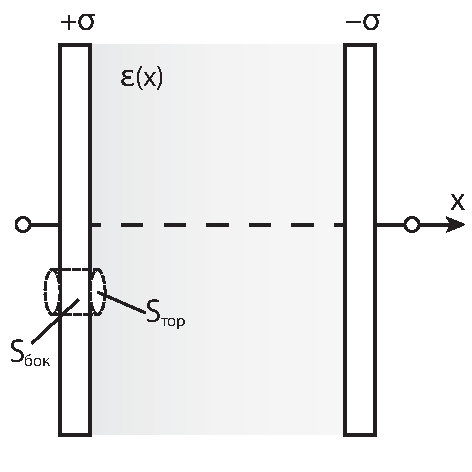
\includegraphics[width=\textwidth]{3-1}
\end{minipage}
\begin{minipage}{.55\textwidth}

Поля \( \vec{E} \) и \( \vec{D} \), в силу симметрии задачи, имеют только одну
компоненту и направлены вдоль оси \( x \).

Окружим малый участок пластины замкнутой цилиндрической поверхностью.
Запишем теорему Гаусса для \( \vec{D} \):
\[
    \oiint\limits_S \vec{D}\d\vec{S} = \sigma S_\emph{н.тор}
\]
\end{minipage}

Первый интеграл можно расписать следующим образом:
\[
    \oiint\limits_S \vec{D}\d\vec{S} = \iint\limits_{S_\emph{бок}} \vec{D}
    \d\vec{S} + \iint\limits_{S_\emph{н.тор}} \vec{D}\d\vec{S} +
    \iint\limits_{S_\emph{в.тор}} \vec{D}\d\vec{S}.
\]

Так как вне конденсатора поля нет, то \( \ds \iint\limits_{S_\emph{в.тор}}
\vec{D}\d\vec{S} = 0 \). Поле \( \vec{D} \) сонаправлено с осью \( x \),
следовательно, \( \ds \iint\limits_{S_\emph{бок}} \vec{D}\d\vec{S} = 0 \).

Тогда
\[
    \sigma S_\emph{н.тор} = \iint\limits_{S_\emph{н.тор}} \vec{D}\d\vec{S} =
    D\iint\limits_{S_\emph{н.тор}} dS = DS_\emph{н.тор},
\]
откуда \( D = \sigma \). С другой стороны \( D = \eps\Ezero E \), откуда
\( E = \cfrac{\sigma}{\eps\Ezero} \).

\vspace*{2em}
\emph{Ответ:} \( \vec{E} = \cfrac{\sigma}{\eps\Ezero}\,\vec{e}_x \).

\newpage
%-------------------------------------------------------------------------------
Задача 1.58: \emph{Вычислить емкость цилиндрического конденсатора. Длина его
\( l \), радиусы обкладок \( R_1 \) и \( R_2 \). Между обкладками два
коаксиальных слоя однородных диэлектриков с проницаемостью \( \eps_1 \) и
\( \eps_2 \), граница раздела между ними -- цилиндрическая поверхность радиуса
\( R_0 \). Краевым эффектом пренебречь.}

\vspace*{2em}
\emph{Решение:}

\begin{minipage}{.4\textwidth}
    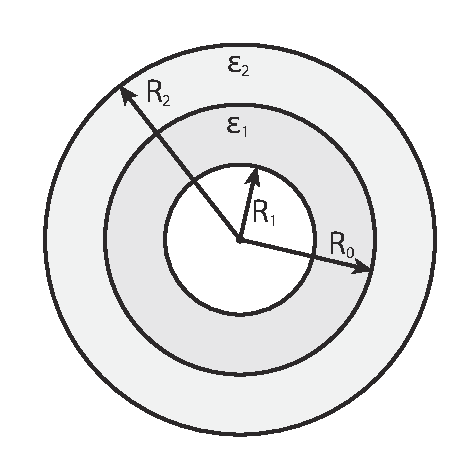
\includegraphics[width=\textwidth]{3-2}
\end{minipage}
\begin{minipage}{.55\textwidth}
    Пусть конденсатор заряжен с погонным зарядом \( \gamma = q/2\pi r \).
    
    Поле \( \vec{E} \) между обкладками создается только внутренним цилиндром
    \[
        E(r)\Bigr|_{R_1 < r < R_2} = \frac{\gamma}{2\pi\eps\Ezero r}\biggr|_{R_1 < r < R_2}.
    \]
    
    По теореме Гаусса:
    \[
        \oiint\limits_S \vec{E}\d\vec{S} = \frac{q}{\eps\Ezero}
    \]
\end{minipage}
    
Первый интеграл можно расписать следующим образом:
\[
    \oiint\limits_S \vec{E}\d\vec{S} = \iint\limits_{S_\emph{бок}} \vec{E}
    \d\vec{S} + 2\iint\limits_{S_\emph{тор}} \vec{E}\d\vec{S}.
\]
Так как поле \( \vec{E} \uparrow\uparrow \vec{n}_\emph{бок} \), то
\( \ds \iint\limits_{S_\emph{тор}} \vec{E}\d\vec{S} = 0 \) и
\( \ds \iint\limits_{S_\emph{бок}} \vec{E}\d\vec{S} =
E\iint\limits_{S_\emph{бок}} dS = 2\pi rlE \).

Тогда поле \( E = \cfrac{q}{2\pi rl \eps\Ezero} \), и разность потенциалов:
\begin{gather*}
    \Delta\phi = \int\limits_{R_1}^{R_2} E\,dr = \frac{q}{2\pi\Ezero l}\left(
    \int\limits_{R_1}^{R_0} \frac{dr}{\eps_1r} + \int\limits_{R_0}^{R_2} \frac{dr}
    {\eps_2r}\right) = \frac{q}{2\pi\Ezero l}\left(\frac{1}{\eps_1} \ln R
    \biggr|_{R_1}^{R_0} + \frac{1}{\eps_2}\ln R\biggr|_{R_0}^{R_2}\right) = \\
    = \frac{q}{2\pi\Ezero l}\left(\frac{1}{\eps_1}\ln\frac{R_0}{R_1} +
    \frac{1}{\eps_2}\ln\frac{R_2}{R_0}\right).
\end{gather*}

Тогда емкость цилиндрического конденсатора: \( \ds C = \frac{q}{\Delta\phi} =
\frac{2\pi\Ezero l}{\left(\frac{1}{\eps_1}\ln\frac{R_0}{R_1} + \frac{1}{\eps_2}
\ln\frac{R_2}{R_0}\right)} \).

\emph{Ответ:} \( \ds C =\frac{2\pi\Ezero l}{\left(\frac{1}{\eps_1}
\ln\frac{R_0}{R_1} + \frac{1}{\eps_2}\ln\frac{R_2}{R_0}\right)} \).

\newpage
%-------------------------------------------------------------------------------
Задача 1.115: \emph{В вакууме имеется бесконечно длинный заземленный проводящий
круглый цилиндр радиуса \( a \). Параллельно его оси протянута нить на
расстоянии \( l > a \) от нее. Нить равномерно заряжена с линейной плотностью
\( \chi \). Определить создаваемое ею поле и силу, действующую на единицу длины
нити.}

\vspace*{2em}
\emph{Решение:}

\begin{minipage}{.4\textwidth}
    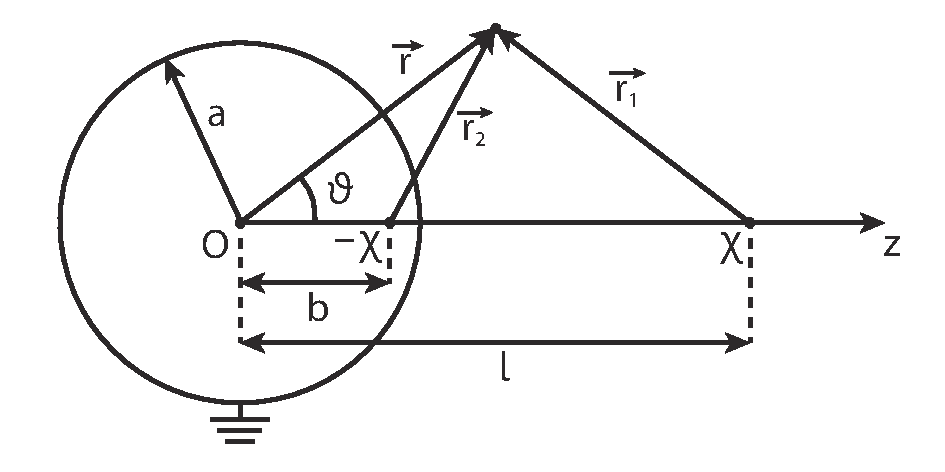
\includegraphics[width=\textwidth]{3-3}
\end{minipage}
\begin{minipage}{.55\textwidth}
\end{minipage}

\vspace*{2em}
\emph{Ответ:}

\newpage
%-------------------------------------------------------------------------------
Задача 2.33: \emph{Однородный магнетик имеет форму бесконечно длинного
круглого цилиндра радиуса \( a \), магнитная проницаемость его \( \mu \);
окружающая среда -- воздух. Бесконечный прямолинейный ток проходит в воздухе
параллельно оси магнетика на расстоянии \( l \) от нее. Определить создаваемое
им магнитное поле.}

\vspace*{2em}
\emph{Решение:}

\begin{minipage}{.4\textwidth}
    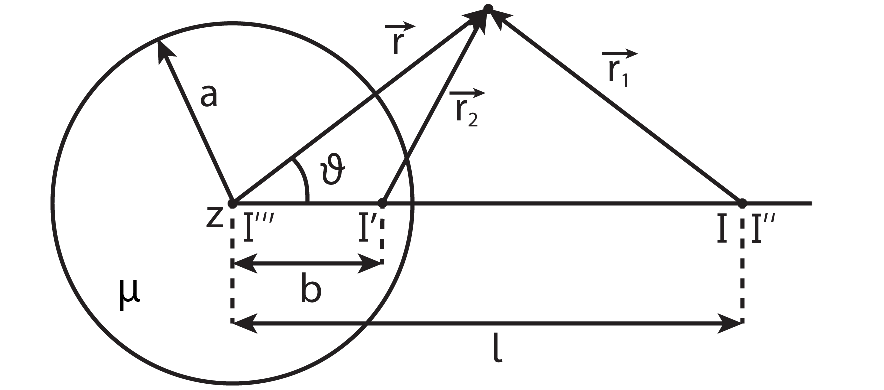
\includegraphics[width=\textwidth]{3-4}
\end{minipage}
\begin{minipage}{.55\textwidth}
\end{minipage}

\vspace*{2em}
\emph{Ответ:}

\end{document}
